\documentclass{beamer}

\useoutertheme{infolines}

\setbeamersize{
  text margin left = 1cm,
  text margin right = 1cm,
}

\setbeamertemplate{frametitle}[default][right]
\setbeamertemplate{navigation symbols}{}

\AtBeginPart{\frame{\partpage}}

\title[Streaming Algorithms]{Theory and Proof-of-Concept Implementations \\ of Streaming Algorithms for Multiset Data}
\subtitle{MSc Computer Science Conversion Project}
\author{Martin de Spirlet}
\institute[]{University of Birmingham}
\date{Project Presentation}

\usepackage{adjustbox} % Graphics package-alike macros for “general” boxes
\usepackage{algpseudocode} % Pseudocode environments for use with the `algorithmicx' style
\usepackage{centernot} % Centred \not command
\usepackage{forest} % Drawing (linguistic) trees
\usepackage{mathtools} % Mathematical tools to use with amsmath
\usepackage{stmaryrd} % St Mary Road symbols for theoretical computer science

% Define algorithmic condition text
\algnewcommand{\algorithmicconstant}{\textbf{constant:}}
\algnewcommand{\algorithmicin}{\textbf{in:}}
\algnewcommand{\algorithmiclocal}{\textbf{local:}}
\algnewcommand{\algorithmicout}{\textbf{out:}}

% Define algorithmic conditions
\algnewcommand{\Constant}{\item[\algorithmicconstant]}
\algnewcommand{\In}{\item[\algorithmicin]}
\algnewcommand{\Local}{\item[\algorithmiclocal]}
\algnewcommand{\Out}{\item[\algorithmicout]}

% Define algorithmic keyword text
\algnewcommand{\algorithmiccopy}{\textbf{copy}}
\algnewcommand{\algorithmicdiv}{\textbf{div}}
\algnewcommand{\algorithmicdownto}{\textbf{down to}}
\algnewcommand{\algorithmicland}{\textbf{and}}
\algnewcommand{\algorithmiclforall}{\textbf{for all}}
\algnewcommand{\algorithmicmod}{\textbf{mod}}
\algnewcommand{\algorithmicto}{\textbf{to}}

% Define algorithmic keywords
\newcommand*{\binarykeyword}[1]{\ifmmode\thickspace#1\thickspace\else#1\fi}
\newcommand*{\unarykeyword}[1]{#1\ifmmode\medspace\fi}
\algnewcommand{\Copy}{\unarykeyword{\algorithmiccopy}}
\algnewcommand{\Div}{\binarykeyword{\algorithmicdiv}}
\algnewcommand{\DownTo}{\binarykeyword{\algorithmicdownto}}
\algnewcommand{\LAnd}{\binarykeyword{\algorithmicland}}
\algnewcommand{\LForAll}{\binarykeyword{\algorithmiclforall}}
\algnewcommand{\Mod}{\binarykeyword{\algorithmicmod}}
\algnewcommand{\To}{\binarykeyword{\algorithmicto}}

% Define algorithmic literal text
\algnewcommand{\algorithmicfalse}{false}
\algnewcommand{\algorithmictrue}{true}

% Define algorithmic literals
\newcommand*{\literal}[1]{\textproc{#1}}
\algnewcommand{\False}{\literal{\algorithmicfalse}}
\algnewcommand{\True}{\literal{\algorithmictrue}}

% Define algorithmic primitives
\newcommand*{\primitive}[1]{\textit{#1}\ifmmode\thinspace\fi}
\newcommand*{\base}{\primitive{base}}
\newcommand*{\discriminatorFunction}{\primitive{discriminatorFunction}}
\newcommand*{\discriminatorFunctions}{\primitive{discriminatorFunctions}}
\newcommand*{\hashFunction}{\primitive{hashFunction}}
\newcommand*{\hashFunctions}{\primitive{hashFunctions}}

% Define command for relaxed math mode
\newcommand*{\relaxedmath}[1]{\(#1\)\relax}

% Define commands for delimited data structures
\newcommand*{\suchthat}{}
\DeclarePairedDelimiter{\dataarray}{\lbrack}{\rbrack}
\DeclarePairedDelimiter{\dataintegerinterval}{\llbracket}{\rrbracket}
\DeclarePairedDelimiterX{\datamultiset}[1]{\lbrace}{\rbrace}{\renewcommand*{\suchthat}{\suchthatsymbol[\delimsize]}#1}
\DeclarePairedDelimiter{\datasequence}{\langle}{\rangle}
\DeclarePairedDelimiterX{\dataset}[1]{\lbrace}{\rbrace}{\renewcommand*{\suchthat}{\suchthatsymbol[\delimsize]}#1}

% Define commands for delimited operations
\DeclarePairedDelimiter{\absolute}{\lvert}{\rvert}
\DeclarePairedDelimiter{\cardinality}{\lvert}{\rvert}
\DeclarePairedDelimiter{\ceiling}{\lceil}{\rceil}
\DeclarePairedDelimiter{\floor}{\lfloor}{\rfloor}
\DeclarePairedDelimiterXPP{\norm}[1]{}{\lVert}{\rVert}{}{#1}
\DeclarePairedDelimiterXPP{\lnorm}[2]{}{\lVert}{\rVert}{_{#1}}{#2}

% Define commands for functions
\newcommand*{\given}{}
\DeclarePairedDelimiterXPP{\bigo}[1]{O}{\lparen}{\rparen}{}{#1}
\DeclareMathOperator{\expectation}{E}
\DeclareMathOperator{\indicator}{\mathbf{1}}
\DeclareMathOperator*{\mean}{mean}
\DeclareMathOperator*{\median}{median}
\DeclareMathOperator{\probability}{\Pr}
% \DeclarePairedDelimiterXPP{\probability}[1]{\Pr}{\lparen}{\rparen}{}{\renewcommand*{\given}{\givensymbol[\delimsize]}#1}

% Define commands for sets of numbers
\newcommand*{\integers}{\mathbb{Z}}
\newcommand*{\nonnegativeintegers}{\mathbb{Z}_{0}^{+}}
\newcommand*{\positiveintegers}{\mathbb{Z}^{+}}
\newcommand*{\primes}{\mathbb{P}}
\newcommand*{\realnumbers}{\mathbb{R}}

% Define commands for styles
\newcommand*{\mathvector}[1]{\mathbf{#1}}

% Define commands for symbols
\newcommand*{\givensymbol}[1][]{\nonscript\medspace#1\vert\allowbreak\nonscript\medspace\mathopen{}}
\newcommand*{\niff}{\centernot\iff}
\newcommand*{\suchthatsymbol}[1][]{\nonscript\medspace#1\vert\allowbreak\nonscript\medspace\mathopen{}}


\begin{document}

\begin{frame}
  \titlepage
\end{frame}

\begin{frame}
  \frametitle{Outline}

  \uncover<1->{\tableofcontents[part=1]}
  \uncover<2->{\tableofcontents[part=2]}
  \uncover<3->{\tableofcontents[part=3,hideallsubsections]}
  \uncover<4->{\tableofcontents[part=4,hideallsubsections]}
\end{frame}

\chapter{Introduction}
\label{ch:introduction}

\section{Background}
\label{sec:introduction-background}

As a civilization, humanity generates and captures a vast quantity of data.
This quantity is growing at an exponential rate, due not only to the proliferation of technologies such as ubiquitous computing, social media and the Internet of Things, but also to humankind's insatiable thirst for knowledge, which has been growing steadily ever since man first looked up at the stars and pondered his place in the universe.
Indeed, while the Very Large Array radio telescope currently collects hundreds of terabytes of astronomical data each year~\citep{choi20}, when the Square Kilometre Array becomes operational in 2024, it will be able to collect up to \num{14}~exabytes of data~\citep{francis12} and store two~petabytes of it every day~\citep{choi20}.
The storage and processing of such cosmic volumes of data presents obvious problems, not least because they are far in excess of what is economically feasible to store for any extended period of time.
Moreover, the global capacity for the generation of data is increasing at a far greater rate than the global capacity for its storage~\citep{cormode20}.
For example, the global computational capacity per capita doubled roughly every \num{18}~months between 1986 and 2007, whereas the global data storage capacity per capita doubled roughly every \num{40}~months during the same period~\citep{hilbert11}.
The field of data science that concerns the analysis and management of data that are too vast to process via traditional methods is known as `big data'~\citep{ibm20}.
Other sources of big data include the sequencing of genomes, which are approximately one~gigabyte per person~\citep{cormode20}, the diagnosis of medical conditions using machine learning, which requires the processing of high-resolution uncompressed images~\citep{yanase19}, and the tracking of social interactions and consumer activity~\citep{ibm20}.

One solution to the problem of processing big data is the paradigm of \emph{streaming algorithms}.
In this paradigm, data is represented as a stream of arbitrary length and arbitrary order~\citep{cormode20}.
Streaming algorithms are used to construct \emph{summaries} of the data by considering each element one at a time.
The summaries are designed to be significantly more compact than a representation of the data in its entirety.
Often, a summary consists of only a handful of properties or a reduced array of the data, which is known as a `sketch'~\citep{babcock02}.
Because a summary is so much more compact than the data from which it is built, the properties of the data that it maintains tend to be approximations rather than exact values.
Additionally, since not all of the data is stored, only certain properties can be maintained by any particular summary.
Nevertheless, since the compact summary is all that must be processed in order to honour a query regarding the original data with an approximate result, this takes significantly less time than the traditional approach of computing the result by storing and processing the data in its entirety, particularly since, in order to compute the updated values of properties, the latter approach often requires all the data to be reprocessed if a change is made to them~\citep{cormode20}.
Different types of summary can be constructed in order to query different properties of data.

A streaming algorithm is a type of online algorithm; it processes its input data one item at a time before the data is available in its entirety.
The class of online algorithms provides solutions to the class of dynamic problems, for which efficient algorithms and data structures are used to compute properties of data whenever it changes~\citep{karp92}.
Another type of online algorithm is the dynamic algorithm, which provides a solution to a dynamic problem with efficient time complexity, whereas a streaming algorithm provides a solution with efficient space complexity~\citep{demetrescu10}.
Streaming algorithms are useful in applications that deal with large and constantly changing data, where it is not necessary to retain data after computing a result---data locality, or where approximation is permitted or even desired.
For example, they can be used to compute queries and joins in databases~\citep{karp87}, to detect distributed denial-of-service attacks~\citep{liu11}, and to implement \emph{differential privacy}---the publication of otherwise private data in a reduced and anonymous form~\citep{cormode12}.
Typically, the data in question are constantly changing in real time.
In the traditional paradigm, supporting changes to the data being queried often requires storing or reprocessing the data in its entirety.
For example, the traditional approach to supporting queries on the ranks of arbitrary elements in the data would involve constructing a frequency table over the data, updating it every time the data changes, and computing the rank of a given element as the sum of the frequencies of all elements less than it.
For large datasets, this is inefficient in terms of both space and time.

A streaming algorithm provides the ability to update and query data efficiently at any time without having to reprocess all of the previously encountered data.
This is achieved by ensuring that its summary update operation is commutative.
This allows a summary to be easily updated given only its current value and the next datum in the stream, and also ensures that the value of a summary is independent of the order in which the data appear in the stream.
Another useful property arising from the use of commutative operations is that two summaries computed using the same commutative operation can often be combined into a single summary using that same operation.
This allows summaries of distinct portions of data to be computed concurrently and eventually combined in order to obtain a summary of the data in its entirety~\citep{cormode20}.

It could be argued that the most basic streaming algorithm is summation, which uses the commutative update operation of addition to produce a sum as its single-valued summary.
Another trivial streaming algorithm is the \emph{moving average}.
By maintaining the current arithmetic mean \( \overline{x}_{n} \) and the number of items \( n \) processed so far, it is possible to compute the arithmetic mean \( \overline{x}_{n + 1} \) of the union of the \( n \) previous items and item~\( (n + 1) \) without storing any of the items from the stream, as formalized in \cref{eq:introduction-background-moving-average}.
The streaming algorithms studied in this project are significantly more substantial than these, however.

\begin{equation}
  \label{eq:introduction-background-moving-average}
  \overline{x}_{n + 1} = \frac{\overline{x}_{n} + x_{n + 1}}{n + 1}
\end{equation}


\section{Aims and Objectives}
\label{sec:introduction-aims}

The aims of this project are to investigate streaming algorithms, specifically those of the fingerprint summary, count sketch and dyadic count sketch, and to implement these algorithms to create an extensible library as proof of concept.
In particular, the algorithms are to be understood theoretically, expressed formally in pseudocode, and analysed in order to reason about their correctness.
Additionally, they are to be implemented in Java, and their performance and accuracy are to be evaluated on carefully designed artificial datasets.
The results are to be analysed with respect to relevant literature and the properties of the datasets used.

All three of the summaries chosen for this project concern multiset data, for which each datum in a stream is an ordered pair of an integer item and a weight.
Each weight is interpreted as a summand of the multiplicity of its corresponding item in the underlying multiset of the stream.
The multiset representation of data is useful due to the common occurrence of data in which each item is mapped to a quality, which could be interpreted as a frequency, weight or other useful value~\citep{singh07}.
All three summaries accept both positive and negative weights, which represent the insertion and removal of items to and from the multiset, respectively.
The dyadic count sketch has a restriction, however, that for the error bound described in \cref{subsec:dyadic-count-sketch-analysis-accuracy} to hold, the overall multiplicity of each item in the multiset must be non-negative when the summary is queried.

The fingerprint summary represents a multiset as a single compact hash value, such that two fingerprint summaries can be compared for equality in order to determine whether they represent the same multiset~\citep{cormode20}.
In this text, a summary of this type is said to belong to the class of `identification' summaries.
The count sketch represents a multiset as a compact array of counters, such that it can be queried for the approximate multiplicity (frequency) of a given item in the underlying multiset of the stream~\citep{charikar02}.
In this text, a summary of this type is said to belong to the class of `frequency' summaries.
The dyadic count sketch represents a multiset as a dyadic structure of frequency summaries, such that it can be queried for the approximate rank of a given item in the underlying multiset of the stream---a \emph{rank} query, or for an item of approximately the given rank---a \emph{quantile} query~\citep{cormode05}.
Thus, in this text, the dyadic count sketch is said to belong both to the class of `rank' summaries and to that of `quantile' summaries.

The topic of streaming algorithms was chosen for this project because it appeared to be challenging and stimulating, especially as the author had no prior knowledge or experience of the subject, and only introductory knowledge of the field of algorithms and complexity.
The fingerprint summary and dyadic count sketch were chosen specifically because these summaries do not have many implementations conveniently available online.
This is particularly true of the dyadic count sketch, to the extent that one of its authors recently noted that it had not yet attracted \emph{any} such implementations~\citep{cormode20}.
Although the count sketch has more available implementations than the other two summaries, its choice was necessitated by the use of the count sketch as a frequency summary in the dyadic count sketch.
The rationales behind some of the more interesting decisions made throughout the project are described in \cref{ch:discussion}.

Among the original contributions of this project are the implementation library and the evaluations performed on it.
The library has been designed with usability and best practices in mind, although it should be noted that due to the theoretical nature of the project, i.e.\@ the library is intended as a proof of concept rather than a robust tool for use in industry, little emphasis is placed on such practical concerns in this text.
For example, such tasks as the gathering of user requirements and the design of unit tests have been omitted, as these are not within the scope of the theoretical approach.
Indeed, the unit testing of the streaming algorithms is not required, as the correctness of the preconditions and postconditions are verified via theoretical analysis before the algorithms are implemented.

Another contribution of this project is the understanding of streaming algorithms presented in this text.
In many cases, this is simply a more digestible---but no less detailed---depiction of the theory presented in the definitive literature.
Nevertheless, the work does include some original analyses that compare the summaries to their traditional counterparts, and determine whether and, if so, how the universes from which items and weights are drawn can be extended beyond those discussed in their definitions.
Such analyses do not appear prevalent in published literature concerning streaming algorithms.


\begin{forest}
  for tree = {
    draw,
    folder,
    grow' = 0,
  }
  [/
    [docs]
    [src
      [lib
        [src
          [main]
          [test]
        ]
        [build.gradle]
      ]
      [gradlew]
      [gradlew.bat]
      [settings.gradle]
    ]
  ]
\end{forest}



\part{The Fingerprint Summary}

\section{The Fingerprint Summary}

\subsection{Overview}

\begin{frame}
  \frametitle{Overview}

  \begin{block}<1->{Identification Summary}
    \begin{itemize}
      \item Represents a stream of arbitrary length as a single compact hash value
      \item Comparison for equality
      \item Non-negative integer item from universe \( U = \dataintegerinterval{u} = \dataintegerinterval{0, u - 1} \)
      \item Positive or negative integer weight
    \end{itemize}
  \end{block}

  \begin{block}<2->{Rolling Hash Function}
    \begin{itemize}
      \item Prime \( p > u - 1 \)
      \item Random base \( \alpha \in \dataintegerinterval{1, p - 1} \)
      \item Maintains hash value \( f \in \dataintegerinterval{0, p - 1} \)
    \end{itemize}
  \end{block}
\end{frame}

\subsection{Applications}

\begin{frame}
  \frametitle{Applications}

  \begin{block}<1->{Equality of Vectors}
    \begin{itemize}
      \item Database queries and joins
      \item Checksums
    \end{itemize}
  \end{block}

  \begin{block}<2->{Similarity of Vectors}
    \begin{itemize}
      \item Search engines
      \item Natural language processing
      \item File diffs
      \item Can be extended to other data types
    \end{itemize}
  \end{block}
\end{frame}

\subsection{Theory}

\begin{frame}
  \frametitle{The Initialization Operation}

  \begin{algorithmic}[1]
  \Out the initial array \( C = \dataarray{0}_{m \times n} \) of counters
  \Constant the number \( m \in \positiveintegers \) of rows in the array; the number \( n \in \positiveintegers \) of columns in the array; the prime number \( p \in \dataset{\phi \in \primes \suchthat \phi > n} \)
  \Local the hash functions \( h_{i} \colon \integers \to \dataintegerinterval{n} \) that each map an item to a position in row~\( i \) of the array; the discriminating hash functions \( g_{i} \colon \integers \to \dataset{-1, +1} \) that each map an item to the sign adjustment of its update in row~\( i \) of the array
  \Function{Initialize}{}
    \State \( C \gets \dataarray{0}_{m \times n} \)
    \ForAll{\( i \in \dataintegerinterval{m} \)}
      \State \( \datasequence{\alpha_{i}, \beta_{i}} \gets \) pick uniformly at random from \( \dataintegerinterval{1, p - 1} \)
      \State \( \hashFunction (C, i) \gets h_{i} \colon x \mapsto ((\alpha_{i} \cdot x + \beta_{i}) \Mod p) \Mod n \)
      \State \( \datasequence{\gamma_{i}, \theta_{i}} \gets \) pick uniformly at random from \( \dataintegerinterval{1, p - 1} \)
      \State \( \discriminatorFunction (C, i) \gets g_{i} \colon x \mapsto 2 \cdot (((\gamma_{i} \cdot x + \theta_{i}) \Mod p) \Mod 2) - 1 \)
    \EndFor
    \State \Return \( C \)
  \EndFunction
\end{algorithmic}

\end{frame}

\begin{frame}
  \frametitle{The Update Operation}

  \begin{algorithmic}[1]
  \In the ordered pair \( \cramped{T \in \integers^{\lambda \times m \times n} \times \integers^{(L - \lambda) \times u / 2^{\lambda}}} \) of arrays of counters and tuples of frequency tables to update; the item \( x \in U \) for which to update the pair; the weight \( w \in \integers \) of the update to the item
  \Out the updated pair \( \cramped{T' \in \integers^{\lambda \times m \times n} \times \integers^{(L - \lambda) \times u / 2^{\lambda}}} \)
  \Constant the number \( L = \ceiling{\lg u} \) of levels in the dyadic structure; the number \( \lambda = \floor{\lg (u / (m \cdot n))} + 1 \) of lower levels in the dyadic structure; the number \( m \in \positiveintegers \) of rows in each array
  \Function{Update}{\relaxedmath{T}, \relaxedmath{x}, \relaxedmath{w}}
    \State \( \datasequence{C, D} \gets T \)
    \State \( \datasequence{C', D'} \gets \Copy \datasequence{C, D} \)
    \For{\( l \gets 0 \To (L - 1) \)}
      \If{\( l < \lambda \)}
        \State \( \hashFunctions (C'_{l}) \gets \hashFunctions (C_{l}) \)
        \State \( \discriminatorFunctions (C'_{l}) \gets \discriminatorFunctions (C_{l}) \)
        \ForAll{\( i \in \dataintegerinterval{m} \)}
          \State \( j \gets (\hashFunction (C'_{l}, i))(x) \)
          \State \( k \gets (\discriminatorFunction (C'_{l}, i))(x) \)
          \State \( (C'_{l})_{i, j} \gets (C'_{l})_{i, j} + k \cdot w \)
        \EndFor
      \Else
        \State \( l' \gets l - \lambda \)
        \State \( (D'_{l'})_{x} \gets (D'_{l'})_{x} + w \)
      \EndIf
      \State \( x \gets x \Div 2 \)
    \EndFor
    \State \( T' \gets \datasequence{C', D'} \)
    \State \Return \( T' \)
  \EndFunction
\end{algorithmic}

\end{frame}

\begin{frame}
  \frametitle{The Merge Operation}

  \begin{algorithmic}[1]
  \In the two arrays \( A, B \in \realnumbers^{m \times n} \) of counters to merge (\( \hashFunctions (A) = \hashFunctions (B) \) \LAnd{} \( \discriminatorFunctions (A) = \discriminatorFunctions (B) \))
  \Out the merged array \( C = \dataarray{A_{i, j} + B_{i, j}}_{m \times n} \in \realnumbers^{m \times n} \)
  \Function{Merge}{\relaxedmath{A}, \relaxedmath{B}}
    \State \( C \gets \dataarray{A_{i, j} + B_{i, j}}_{m \times n} \)
    \State \( \hashFunctions (C) \gets \hashFunctions (A) \)
    \State \( \discriminatorFunctions (C) \gets \discriminatorFunctions (A) \)
    \State \Return \( C \)
  \EndFunction
\end{algorithmic}

\end{frame}

\begin{frame}
  \frametitle{The Query and Equality Operations}

  \begin{block}{Comparisons}
    \begin{itemize}
      \item Query returns hash value
      \item Hash values compared for equality
      \item Assuming two fingerprints have the same base
      \begin{itemize}
        \item multiset equality implies fingerprint equality
        \item fingerprint inequality implies multiset inequality
        \item fingerprint equality does not imply multiset equality
      \end{itemize}
      \item Probability of false positive can be bound
    \end{itemize}
  \end{block}
\end{frame}

\subsection{Analysis}

\begin{frame}
  \frametitle{Accuracy}

  \begin{block}<1->{Polynomial}
    \begin{itemize}
      \item Hash function is a polynomial \( \sum_{x \in U} w_{x} \cdot \alpha^{x} \pmod p \)
      \item At most \( u - 1 \) integer roots \( \alpha \)
    \end{itemize}
  \end{block}

  \begin{block}<2->{Equivalent Tests}
    \begin{itemize}
      \item \( f = f' \iff f - f' = 0 \)
      \item At most \( u - 1 \) integer roots \( \alpha \) where \( f - f' = 0 \)
      \item At most \( u - 1 \) values of \( \alpha \) where \( f = f' \)
      \item False positives or hash collisions
    \end{itemize}
  \end{block}
\end{frame}

\begin{frame}
  \frametitle{Accuracy}

  \begin{block}<1->{Choosing the Base \( \alpha \)}
    \begin{itemize}
      \item At most \( u - 1 \) roots \( \alpha \)
      \item \( \alpha \) is drawn from \( \dataintegerinterval{1, p - 1} \)
      \item Less chance of choosing root if \( p - 1 \gg u - 1 \)
    \end{itemize}
  \end{block}

  \begin{block}<2->{Choosing the Prime \( p \)}
    \begin{itemize}
      \item Choose \( p - 1 \geq (u - 1) / \delta \)
      \item Probability of false positive is at most \( \delta \)
    \end{itemize}
  \end{block}
\end{frame}

\begin{frame}
  \frametitle{Space and Time Complexities}

  \begin{block}{A Traditional Hash Table}
    \begin{itemize}
      \item<alert@2> Space complexity \( \bigo{u} \)
      \item<alert@3> Update time complexity (per datum) \( \bigo{1} \)
      \item<alert@4> Equality time complexity \( \bigo{u} \)
    \end{itemize}
  \end{block}

  \begin{block}{The Fingerprint Summary}
    \begin{itemize}
      \item<alert@2> Space complexity \( \bigo{1} \)
      \item<alert@3> Update time complexity (per datum) \( \bigo{1} \)
      \item<alert@5> Equality time complexity \( \bigo{1} \)
      \item<alert@5> Chance of false positive
    \end{itemize}
  \end{block}
\end{frame}


\part{The Count Sketch}

\section{The Count Sketch}

\subsection{Overview}

\begin{frame}
  \frametitle{Overview}

  \begin{block}<1->{Frequency Summary}
    \begin{itemize}
      \item Represents a stream of arbitrary length as an \( m \times n \) array of counters
      \item Query for approximate frequencies
      \item Positive or negative integer item
      \item Positive or negative real-valued weight
    \end{itemize}
  \end{block}

  \begin{block}<2->{Pairwise Hash Functions}
    \begin{itemize}
      \item Hash function \( h \colon \integers \to \dataintegerinterval{n}; \enspace x \mapsto ((\alpha \cdot x + \beta) \bmod p) \bmod n \)
      \item Discriminating hash function \( g \colon \integers \to \dataset{-1, +1}; \enspace x \mapsto 2 \cdot (((\gamma \cdot x + \theta) \bmod p) \bmod 2) - 1 \)
      \item Pairwise independent
    \end{itemize}
  \end{block}
\end{frame}

\subsection{Applications}

\begin{frame}
  \frametitle{Applications}

  \begin{block}{A Versatile Summary}
    \begin{itemize}
      \item Distributed denial of service
      \begin{itemize}
        \item Detection
        \item Victim tracking
      \end{itemize}
      \item Differential privacy
      \begin{itemize}
        \item Reduced size
        \item Added noise
      \end{itemize}
      \item Compressed matrix multiplication
    \end{itemize}
  \end{block}
\end{frame}

\subsection{Theory}

\begin{frame}
  \frametitle{Example}

  \begin{figure}
    \centering
    \begin{tabular}{|c|c|c|c|c|c|c|}
      \hline
       & \( \action<6->{-}\action<2->{w_{b}} \) &  & \( \action<6->{+}\action<2->{w_{a}} \) &  & \( \action<6->{+}\action<2->{w_{c}} \) &  \\
       &  &  &  &  &  &  \\
      \hline
      \( \action<6->{+}\action<3->{w_{b}} \) &  &  &  & \( \action<6-|alert@1->{-}\action<3-|alert@1->{w_{a}} \) &  &  \\
       &  &  &  & \( \action<6-|alert@1->{-}\action<3-|alert@1->{w_{c}} \) &  &  \\
      \hline
       &  & \( \action<6-|alert@1->{+}\action<1-|alert@1->{w_{a}} \) &  &  &  & \( \action<6->{+}\action<1->{w_{c}} \) \\
       &  & \( \action<6-|alert@1->{-}\action<1-|alert@1->{w_{b}} \) &  &  &  &  \\
      \hline
       & \( \action<6->{+}\action<4->{w_{b}} \) &  & \( \action<6->{-}\action<4->{w_{a}} \) &  & \( \action<6->{-}\action<4->{w_{c}} \) &  \\
       &  &  &  &  &  &  \\
      \hline
       &  &  & \( \action<6->{+}\action<5->{w_{c}} \) &  & \( \action<6->{+}\action<5->{w_{a}} \) & \( \action<6->{-}\action<5->{w_{b}} \) \\
       &  &  &  &  &  &  \\
      \hline
    \end{tabular}
  \end{figure}
\end{frame}

\begin{frame}
  \frametitle{Example}

  \begin{block}<1->{Get counters corresponding to \( a \)}
    \begin{equation*}
      w_{a}, \qquad -w_{a} - w_{c}, \qquad w_{a} - w_{b}, \qquad -w_{a}, \qquad w_{a}
    \end{equation*}
  \end{block}

  \begin{block}<2->{Reapply discriminating hash functions corresponding to \( a \)}
    \begin{equation*}
      w_{a}, \qquad w_{a} + w_{c}, \qquad w_{a} - w_{b}, \qquad w_{a}, \qquad w_{a}
    \end{equation*}
  \end{block}

  \begin{block}<3->{Sort and return the median}
    \begin{equation*}
      w_{a} - w_{b}, \qquad w_{a}, \qquad \alert{w_{a}}, \qquad w_{a}, \qquad w_{a} + w_{c}
    \end{equation*}
  \end{block}
\end{frame}

\subsection{Analysis}

\begin{frame}
  \frametitle{Probability Theory}

  \begin{block}{A Chernoff Bound Argument}
    \begin{itemize}
      \item Probability that the median of \( \bigo{\ln (1 / \delta)} \) estimates is inaccurate has upper bound \( \delta \)
      \begin{multline*}
        \probability \Biggl( \sum_{i} X_{i} \geq \bigo[\bigg]{\ln \frac{1}{\delta}} \Biggr) < \delta, \\
        X_{i} = \begin{cases}
          0 & \text{if estimate~\( i \) is accurate,} \\
          1 & \text{if estimate~\( i \) is inaccurate}
        \end{cases}
      \end{multline*}
    \end{itemize}
  \end{block}
\end{frame}

\begin{frame}
  \frametitle{Accuracy}

  \begin{actionenv}<1->
    \begin{equation*}
      \action<1->{\hat{w}_{x, i} = g_{i} (x) \cdot C_{i, h_{i} (x)}}\action<2->{, \qquad C_{i, h_{i} (x)} = \smashoperator{\sum_{\substack{s \in U \\ h_{i} (s) = h_{i} (x)}}} g_{i} (s) \cdot w_{s}}
    \end{equation*}
  \end{actionenv}

  \begin{actionenv}<2->
    \begin{equation*}
      \hat{w}_{x, i} = \smashoperator{\sum_{\substack{s \in U \\ h_{i} (s) = h_{i} (x)}}} g_{i} (x) \cdot g_{i} (s) \cdot w_{s}
    \end{equation*}
  \end{actionenv}

  \begin{actionenv}<3->
    \begin{equation*}
      \absolute{w_{x} - \hat{w}_{x, i}} = \absolute[\Big]{\smashoperator{\sum_{\substack{s \in U \\ h_{i} (s) = h_{i} (x) \\ s \neq x}}} g_{i} (x) \cdot g_{i} (s) \cdot w_{s}}
    \end{equation*}
  \end{actionenv}
\end{frame}

\begin{frame}
  \frametitle{Accuracy}

  \begin{align*}
    \action<1->{\expectation \bigl( \absolute{w_{x} - \hat{w}_{x, i}} \bigr) &= \expectation \biggl( \absolute[\Big]{\smashoperator{\sum_{\substack{s \in U \\ h_{i} (s) = h_{i} (x) \\ s \neq x}}} g_{i} (x) \cdot g_{i} (s) \cdot w_{s}} \biggr) \\}
    \action<2->{&\leq \smashoperator{\sum_{\substack{s \in U \\ h_{i} (s) = h_{i} (x) \\ s \neq x}}} \expectation \biggl( \absolute[\Big]{g_{i} (x) \cdot g_{i} (s) \cdot w_{s}} \biggr) \\}
    \action<3->{&= \smashoperator{\sum_{\substack{s \in U \\ h_{i} (s) = h_{i} (x) \\ s \neq x}}} \expectation \Bigl( \absolute{w_{s}} \Bigr)}
    \action<4->{= \smashoperator{\sum_{\substack{s \in U \\ h_{i} (s) = h_{i} (x) \\ s \neq x}}} \absolute{w_{s}}}
  \end{align*}
\end{frame}

\begin{frame}
  \frametitle{Accuracy}

  \begin{equation*}
    \action<1->{\expectation \bigl( \absolute{w_{x} - \hat{w}_{x, i}} \bigr) = \smashoperator{\sum_{\substack{s \in U \\ h_{i} (s) = h_{i} (x) \\ s \neq x}}} \absolute{w_{s}} = \frac{1}{n} \cdot \smashoperator{\sum_{\substack{s \in U \\ s \neq x}}} \absolute{w_{s}}}
    \action<2->{\leq \frac{\lnorm{1}{\mathvector{w}}}{n}}
  \end{equation*}

  \begin{block}<2->{Size of the Array}
    \begin{itemize}
      \item \( n = 1 / \varepsilon \) columns
      \item Expected absolute error at most \( \varepsilon \cdot \lnorm{1}{\mathvector{w}} \)
      \item \( m = \ln (1 / \delta) \) rows
      \item Probability median exceeds expected error at most \( \delta \)
    \end{itemize}
  \end{block}
\end{frame}


\chapter{The Dyadic Count Sketch}
\label{ch:dyadic-count-sketch}

\section{Overview}
\label{sec:fingerprint-overview}

A fingerprint summary is a type of identification summary; it represents the underlying multiset---which may be very large---of a stream \( \mathcal{S} \) as a single, much smaller hash value.
This allows two fingerprints to be compared for equality in order to determine whether they represent the same multiset~\citep{breslauer11}.
In this context, each datum in the stream is an ordered pair of a non-negative integer item \( x \), and a (positive or negative) integer weight \( w \).
The underlying multiset \( S \) comprises all items \( x \) that appear in the stream, and each weight \( w \) is a summand of the multiplicity of its corresponding item in the multiset.
The universe \( U \) from which items are drawn is the integer interval \( U = \dataintegerinterval{u} = \dataintegerinterval{0, u - 1} \), where \( u - 1 \) is the greatest possible value that may appear in the stream~\citep{cormode20}.
This is formalized in \cref{eq:fingerprint-overview-multiset,eq:fingerprint-overview-multiplicity}.

\begin{gather}
  \label{eq:fingerprint-overview-multiset}
  S = \datamultiset[\big]{x \in \dataintegerinterval{u} \suchthat x \in \datasequence{x, w}} \quad \forall\ \datasequence{x, w} \in \mathcal{S}. \\
  \label{eq:fingerprint-overview-multiplicity}
  \cardinality[\big]{\datamultiset{s \in S \suchthat s = x}} = \smashoperator{\sum_{\datasequence{s, w} \in \mathcal{S}}} \indicator_{\dataset{x}} (s) \cdot w \quad \forall\ x \in S.
\end{gather}

Since a multiset maps items (or indices) to multiplicities, a multiset can be represented as a vector of multiplicities.
This means that the fingerprint summary is a solution to the problem of testing for the equality of vectors or sets.
This is a common task in computer science~\citep{breslauer11}.
For example, simple database queries are frequently used to search relations for tuples with a subset of attributes that exactly match a set of given values.
Another example of this problem in database management is the computation of joins, for which, again, tuples are found that match exactly according to a subset of their attributes~\citep{karp87}.
The hash value maintained by a fingerprint summary could also be used as a checksum for validating the correct transmission of packets of data~\citep{tridgell96}.
Although the fingerprint summary is used primarily to check for equality between multisets, multiple fingerprints could be used to check for similarity, since two sets with a large number of equal subsets are likely to be similar.
The ability to check for similarity between vectors of data is useful for search engines, natural language processing and the computation of diffs between files~\citep{tridgell96}.
Although the fingerprint summary is designed to represent multisets of integers, it can be adapted to handle any arbitrary type of data, including strings, as long as a suitable hash function can be found to map each distinct datum to a unique non-negative integer hash value (see \cref{subsec:fingerprint-analysis-universe}).

A fingerprint \( f \) represents a multiset as a hash value in the integer interval \( \dataintegerinterval{0, p - 1} \), where \( p \) is a prime number greater than the upper bound \( u - 1 \) of the universe.
The hash value is computed using a rolling hash function.
This means that the hash value is easily updated for a new input, given only the old hash value and the new input~\citep{karp87}.
This is similar to the computation of a moving average.
The computation of the hash value requires a base \( \alpha \) that must be drawn uniformly at random from the integer interval \( \dataintegerinterval{1, p - 1} \).
The base can be interpreted as a property of the fingerprint.
Thus, in the following algorithms, the base of a fingerprint \( f \) is represented by the primitive routine \( \base (f) \).
Each of the following algorithms is either adapted from, or designed according to the description of, the corresponding operation in the definitive literature~\citep{cormode20}.


\section{Theory}
\label{sec:fingerprint-theory}

\begin{algorithm}
  \caption{The fingerprint summary initialization operation}
  \label{alg:fingerprint-theory-initialize}
  \begin{algorithmic}[1]
  \Out the initial array \( C = \dataarray{0}_{m \times n} \) of counters
  \Constant the number \( m \in \positiveintegers \) of rows in the array; the number \( n \in \positiveintegers \) of columns in the array; the prime number \( p \in \dataset{\phi \in \primes \suchthat \phi > n} \)
  \Local the hash functions \( h_{i} \colon \integers \to \dataintegerinterval{n} \) that each map an item to a position in row~\( i \) of the array; the discriminating hash functions \( g_{i} \colon \integers \to \dataset{-1, +1} \) that each map an item to the sign adjustment of its update in row~\( i \) of the array
  \Function{Initialize}{}
    \State \( C \gets \dataarray{0}_{m \times n} \)
    \ForAll{\( i \in \dataintegerinterval{m} \)}
      \State \( \datasequence{\alpha_{i}, \beta_{i}} \gets \) pick uniformly at random from \( \dataintegerinterval{1, p - 1} \)
      \State \( \hashFunction (C, i) \gets h_{i} \colon x \mapsto ((\alpha_{i} \cdot x + \beta_{i}) \Mod p) \Mod n \)
      \State \( \datasequence{\gamma_{i}, \theta_{i}} \gets \) pick uniformly at random from \( \dataintegerinterval{1, p - 1} \)
      \State \( \discriminatorFunction (C, i) \gets g_{i} \colon x \mapsto 2 \cdot (((\gamma_{i} \cdot x + \theta_{i}) \Mod p) \Mod 2) - 1 \)
    \EndFor
    \State \Return \( C \)
  \EndFunction
\end{algorithmic}

\end{algorithm}

The fingerprint initialization operation is presented in \cref{alg:fingerprint-theory-initialize}.
A fingerprint \( f \) is initialized by setting its value to zero, and a base \( \alpha \) is drawn uniformly at random from the integer interval \( \dataintegerinterval{1, p - 1} \).
This is assigned to the primitive routine \( \base (f) \).
It is assumed that the prime number \( p > u - 1 \) has been selected beforehand.

\begin{algorithm}
  \caption{The fingerprint summary update operation}
  \label{alg:fingerprint-theory-update}
  \begin{algorithmic}[1]
  \In the ordered pair \( \cramped{T \in \integers^{\lambda \times m \times n} \times \integers^{(L - \lambda) \times u / 2^{\lambda}}} \) of arrays of counters and tuples of frequency tables to update; the item \( x \in U \) for which to update the pair; the weight \( w \in \integers \) of the update to the item
  \Out the updated pair \( \cramped{T' \in \integers^{\lambda \times m \times n} \times \integers^{(L - \lambda) \times u / 2^{\lambda}}} \)
  \Constant the number \( L = \ceiling{\lg u} \) of levels in the dyadic structure; the number \( \lambda = \floor{\lg (u / (m \cdot n))} + 1 \) of lower levels in the dyadic structure; the number \( m \in \positiveintegers \) of rows in each array
  \Function{Update}{\relaxedmath{T}, \relaxedmath{x}, \relaxedmath{w}}
    \State \( \datasequence{C, D} \gets T \)
    \State \( \datasequence{C', D'} \gets \Copy \datasequence{C, D} \)
    \For{\( l \gets 0 \To (L - 1) \)}
      \If{\( l < \lambda \)}
        \State \( \hashFunctions (C'_{l}) \gets \hashFunctions (C_{l}) \)
        \State \( \discriminatorFunctions (C'_{l}) \gets \discriminatorFunctions (C_{l}) \)
        \ForAll{\( i \in \dataintegerinterval{m} \)}
          \State \( j \gets (\hashFunction (C'_{l}, i))(x) \)
          \State \( k \gets (\discriminatorFunction (C'_{l}, i))(x) \)
          \State \( (C'_{l})_{i, j} \gets (C'_{l})_{i, j} + k \cdot w \)
        \EndFor
      \Else
        \State \( l' \gets l - \lambda \)
        \State \( (D'_{l'})_{x} \gets (D'_{l'})_{x} + w \)
      \EndIf
      \State \( x \gets x \Div 2 \)
    \EndFor
    \State \( T' \gets \datasequence{C', D'} \)
    \State \Return \( T' \)
  \EndFunction
\end{algorithmic}

\end{algorithm}

The fingerprint update operation is presented in \cref{alg:fingerprint-theory-update}.
This operation updates a fingerprint \( f \) so as to include in its representation of the underlying multiset an increase in the multiplicity of an item \( x \) by weight \( w \).
The value of the updated fingerprint \( f' \) is given by \cref{eq:fingerprint-theory-update}.

\begin{equation}
  \label{eq:fingerprint-theory-update}
  f' = \left( f + w \cdot \alpha^{x} \right) \bmod p.
\end{equation}

\begin{algorithm}
  \caption{The fingerprint summary merge operation}
  \label{alg:fingerprint-theory-merge}
  \begin{algorithmic}[1]
  \In the two arrays \( A, B \in \realnumbers^{m \times n} \) of counters to merge (\( \hashFunctions (A) = \hashFunctions (B) \) \LAnd{} \( \discriminatorFunctions (A) = \discriminatorFunctions (B) \))
  \Out the merged array \( C = \dataarray{A_{i, j} + B_{i, j}}_{m \times n} \in \realnumbers^{m \times n} \)
  \Function{Merge}{\relaxedmath{A}, \relaxedmath{B}}
    \State \( C \gets \dataarray{A_{i, j} + B_{i, j}}_{m \times n} \)
    \State \( \hashFunctions (C) \gets \hashFunctions (A) \)
    \State \( \discriminatorFunctions (C) \gets \discriminatorFunctions (A) \)
    \State \Return \( C \)
  \EndFunction
\end{algorithmic}

\end{algorithm}

Two fingerprints can be merged into one.
This operation allows the fingerprint of a stream to be computed in parallel, i.e.\@ fingerprints of distinct portions of a stream can be computed concurrently and eventually combined in order to obtain the fingerprint of the stream as a whole.
The fingerprint merge operation is presented in \cref{alg:fingerprint-theory-merge}.
Merging two fingerprints \( a \) and \( b \) into a single fingerprint \( f \) is a simple case of addition modulo \( p \), as formalized in \cref{eq:fingerprint-theory-merge}, but this will only work if the two fingerprints are computed using the same base.
This should come as no surprise, since it is a generalization of the update operation; an update is the special case of the merger of one fingerprint \( a = f \), whose base is \( \alpha \), and another fingerprint \( b = w \cdot \alpha^{x} \), whose base is also \( \alpha \)---the only difference being that in the case of an update, the fingerprint \( b \) represents a multiset whose underlying set has a cardinality of one.

\begin{equation}
  \label{eq:fingerprint-theory-merge}
  f = \left( a + b \right) \bmod p.
\end{equation}

\begin{algorithm}
  \caption{The fingerprint summary query operation}
  \label{alg:fingerprint-theory-query}
  \begin{algorithmic}[1]
  \In the array \( C \in \realnumbers^{m \times n} \) to query; the item \( x \in U \) whose approximate frequency in the multiset \( S \) to return
  \Out the approximate frequency \( f \in \realnumbers \) of the item in the multiset (\( f \simeq \cardinality{\datamultiset{s \in S \suchthat s = x}} \))
  \Constant the number \( m \in \positiveintegers \) of rows in the array
  \Local the multiset \( F \in \realnumbers^{m} \) of approximate frequencies of the item
  \Function{Query}{\relaxedmath{C}, \relaxedmath{x}}
    \State \( F \gets \varnothing \)
    \ForAll{\( i \in \dataintegerinterval{m} \)}
      \State \( j \gets (\hashFunction (C, i))(x) \)
      \State \( k \gets (\discriminatorFunction (C, i))(x) \)
      \State \( F \gets F \cup \dataset{k \cdot C_{i, j}} \)
    \EndFor
    \State \( f \gets \median F \)
    \State \Return \( f \)
  \EndFunction
\end{algorithmic}

\end{algorithm}

For the sake of completeness, the fingerprint query operation is presented in \cref{alg:fingerprint-theory-query}.
This operation simply returns the value of the fingerprint.
To approximate whether two fingerprints represent the same multiset, their values can be compared for equality, but this will only work if the two fingerprints are computed using the same base.
If the fingerprints differ, the multisets they represent must also differ.
Additionally, if the multisets are equal, their fingerprints must also be equal.
This is formalized in \cref{eq:fingerprint-theory-unequal-implication,eq:fingerprint-theory-equal-implication}.
Note that if the fingerprints are equal, it is not necessarily the case that the multisets are equal, although for sufficiently large values of \( p \), it is highly likely that they are (see \cref{subsec:fingerprint-analysis-accuracy}).

\begin{align}
  \label{eq:fingerprint-theory-unequal-implication}
  a \neq b \implies S_{a} \neq S_{b}. \\
  \label{eq:fingerprint-theory-equal-implication}
  a = b \impliedby S_{a} = S_{b}.
\end{align}

\begin{algorithm}
  \caption{The fingerprint summary equality operation}
  \label{alg:fingerprint-theory-equal}
  \begin{algorithmic}[1]
  \In the two fingerprints \( a, b \in \dataintegerinterval{0, p - 1} \) to compare (\( \base (a) = \base (b) \))
  \Out whether the fingerprints appear to represent the same multiset \( S \) (\( a \neq b \implies S_{a} \neq S_{b} \) \LAnd{} \( a = b \impliedby S_{a} = S_{b} \))
  \Function{Equal}{\relaxedmath{a}, \relaxedmath{b}}
    \State \Return \( a = b \)
  \EndFunction
\end{algorithmic}

\end{algorithm}

A fingerprint equality operation can be defined for this comparison, as presented in \cref{alg:fingerprint-theory-equal}.
This operation simply returns \True{} if the two fingerprints are equal, and \False{} otherwise.
It is assumed that the fingerprints share the same base.


\section{Analysis}
\label{sec:dyadic-count-sketch-analysis}

\subsection{Accuracy}
\label{subsec:dyadic-count-sketch-analysis-accuracy}

If each constituent count sketch is initialized with \( m = \lg (\lg (u) / \varepsilon) \) rows and \( n = (1 / \varepsilon) \cdot \sqrt{\lg (u) \cdot \lg (\lg (u) / \varepsilon)} \) columns for some error parameter \( \varepsilon \), each approximate rank returned by the dyadic count sketch is guaranteed with constant probability to have an absolute error no greater than \( \varepsilon \cdot \cardinality{S} \)~\citep{cormode20}, where \( \cardinality{S} \) is the cardinality of the underlying multiset \( S \) of the stream.
Although any frequency summary could be used in place of the count sketch, this error bound is particular to the count sketch and makes use of the fact that it returns an unbiased estimator (see \cref{subsec:count-sketch-analysis-accuracy}).
Since the query operations compute the sum of multiple count sketch estimates, this property prevents the accumulation of errors that would be prevalent if a biased frequency summary, such as the count-min sketch, were used instead~\citep{cormode20}.
For the error bound to hold, the multiplicity of each item in the multiset when the summary is queried must be non-negative.
For target ranks \( t \geq \cardinality{S} \), the item returned is the greatest in the multiset \( S \).

\subsection{Space and Time Complexities}
\label{subsec:dyadic-count-sketch-analysis-complexity}

A dyadic count sketch maintains \( l \) levels of frequency summaries.
The frequency summaries of the \( \floor{\lg (u / (m \cdot n))} + 1 \) lower levels are each a count sketch of size \( m \times n \).
For each of the remaining upper levels, the size \( u / 2^{l} \) of the reduced domain of \( U \) is less than the size \( m \cdot n \) of a count sketch, so a frequency table of size \( u /2^{l} \) is used instead.
Thus, the overall space complexity of a dyadic count sketch is \( \bigo{\lg (u) \cdot m \cdot n} \).
By substituting the ideal values of \( m \) and \( n \) given in \cref{subsec:dyadic-count-sketch-analysis-accuracy}, the space complexity of the dyadic count sketch is given by \cref{eq:dyadic-count-sketch-analysis-complexity-space}.

\begin{equation}
  \label{eq:dyadic-count-sketch-analysis-complexity-space}
  \begin{split}
    \bigo[\big]{\lg (u) \cdot m \cdot n} &= \bigo[\Bigg]{\lg (u) \cdot \lg \biggl( \frac{\lg u}{\varepsilon} \biggr) \cdot \frac{1}{\varepsilon} \cdot \sqrt{\lg (u) \cdot \lg \biggl( \frac{\lg u}{\varepsilon} \biggr)}} \\
    &= \bigo[\Bigg]{\frac{1}{\varepsilon} \cdot \lg (u) \cdot \lg \biggl( \frac{\lg u}{\varepsilon} \biggr) \cdot \lg^{\frac{1}{2}} (u) \cdot \lg^{\frac{1}{2}} \biggl( \frac{\lg u}{\varepsilon} \biggr)} \\
    &= \bigo[\Bigg]{\frac{1}{\varepsilon} \cdot \lg^{\frac{3}{2}} (u) \cdot \lg^{\frac{3}{2}} \biggl( \frac{\lg u}{\varepsilon} \biggr)}.
  \end{split}
\end{equation}

Since a count sketch has a greater time complexity than a frequency table for each of its operations, the time complexities of the dyadic count sketch operations are determined by those of the count sketch.
Thus, the time complexities of the dyadic count sketch initialization, update, merge, rank query and quantile query operations are \( \bigo{\lg (u) \cdot m \cdot n} \), \( \bigo{\lg (u) \cdot m} \), \( \bigo{\lg (u) \cdot m \cdot n} \), \( \bigo{\lg (u) \cdot m \cdot \log (m)} \) and \( \bigo{\lg (u) \cdot m \cdot \log (m)} \), respectively (see \cref{subsec:count-sketch-analysis-complexity}).

It would be useful to compare the dyadic count sketch to a more traditional solution that does not originate from the streaming algorithm paradigm.
Such a solution could be a hash table or associative array, in which each entry is a key--value pair of an item in the universe and either its multiplicity or its rank in the underlying multiset of the stream.
Both of these solutions would have a space complexity of \( \bigo{u} \).
The former would have an update time complexity of \( \bigo{1} \), as only one entry must be updated for each datum in the stream, and a query time complexity of \( \bigo{u} \), as the rank of an item must be computed as the sum of the multiplicities of all items less than it.
The latter would have an update time complexity of \( \bigo{u} \), as the ranks of all items greater than the given item must be updated for each datum in the stream, and a query time complexity of \( \bigo{1} \), as the rank of an item is simply returned from the corresponding entry.
Using the ideal values of \( m = \lg (\lg (u) / \varepsilon) \) and \( n = (1 / \varepsilon) \cdot \sqrt{\lg (u) \cdot \lg (\lg (u) / \varepsilon)} \), it is clear that a dyadic count sketch is significantly more compact and offers a good compromise between the time complexities of the update and query operations.

\subsection{Domain of the Universe}
\label{subsec:dyadic-count-sketch-analysis-universe}

As it stands, the current definition of the dyadic count sketch requires that the items in the stream be drawn from the positive integer universe \( U = \dataintegerinterval{u} = \dataintegerinterval{0, u - 1} \)~\citep{cormode20}.
By altering its operations, however, it is permissible for items to be drawn from an extended positive \emph{and} negative universe \( V = \dataintegerinterval{-u, u - 1} \).
The rank of an item in the underlying multiset is still a zero-based standard competition rank that follows the natural order of the integer items of the universe, i.e.\@ the rank of an item in the multiset is the sum of the multiplicities of all items less than it.
This extended universe contains twice as many values as the standard universe.
Therefore, the dyadic count sketch requires an additional level at the bottom of its dyadic structure.
This becomes the new level~\( 0 \).
Since each level represents a dyadic interval of the universe, the additional level is indexed over a domain twice the size of that of the level immediately above it.

\begin{figure}
  \centering
  \begin{forest}
  for tree = {
    align = center,
  },
  [,phantom
    [\( \dataintegerinterval{-4, -1} \) \\ \scriptsize{\( -1 \)}
      [\( \dataintegerinterval{-4, -3} \) \\ \scriptsize{\( -2 \)}
        [\( \dataset{-4} \) \\ \scriptsize{\( -4 \)}]
        [\( \dataset{-3} \) \\ \scriptsize{\( -3 \)}]
      ]
      [\( \dataintegerinterval{-2, -1} \) \\ \scriptsize{\( -1 \)}
        [\( \dataset{-2} \) \\ \scriptsize{\( -2 \)}]
        [\( \dataset{-1} \) \\ \scriptsize{\( -1 \)}]
      ]
    ]
    [\( \dataintegerinterval{0, 3} \) \\ \scriptsize{\( 0 \)}
      [\( \dataintegerinterval{0, 1} \) \\ \scriptsize{\( 0 \)}
        [\( \dataset{0} \) \\ \scriptsize{\( 0 \)}]
        [\( \dataset{1} \) \\ \scriptsize{\( 1 \)}]
      ]
      [\( \dataintegerinterval{2, 3} \) \\ \scriptsize{\( 1 \)}
        [\( \dataset{2} \) \\ \scriptsize{\( 2 \)}]
        [\( \dataset{3} \) \\ \scriptsize{\( 3 \)}]
      ]
    ]
  ]
\end{forest}
%
  \caption{The dyadic intervals of extended universe \( V = \dataintegerinterval{-u, u - 1} = \dataintegerinterval{-4, 3} \)}
  \label{fig:dyadic-count-sketch-analysis-universe-extended-binary-tree}
\end{figure}

The extended dyadic structure comprises \( L = \ceiling{\lg (2 \cdot u)} = \ceiling{\lg u} + 1 \) levels, of which \( \lambda = \floor{\lg (2 \cdot u / (m \cdot n))} + 1 = \floor{\lg (u / (m \cdot n))} + 2 \) are lower levels.
Each level \( l \) is indexed over a reduced domain of \( V \), given by \( \dataintegerinterval{-u / 2^{l}, u / 2^{l} - 1} \), and each of the indices \( v \in \dataintegerinterval{-u / 2^{l}, u / 2^{l} - 1} \) can be mapped to and from a dyadic interval of \( V \), given by \( \dataintegerinterval{v \cdot 2^{l}, (v + 1) \cdot 2^{l} - 1} \).
As with the standard dyadic structure, the reduced domain at level~\( 0 \) is the universe \( V \) itself, and each index in \( V \) is mapped to a singleton set containing itself.
At level~\( L - 1 \), however, the reduced domain of the extended universe is \( \datamultiset{-1, 0} \), and these two indices are mapped to the dyadic intervals \( \dataintegerinterval{-u, -1} \) and \( \dataintegerinterval{0, u - 1} \), respectively.
The binary tree formed from the dyadic intervals of \( V \) is shown in \cref{fig:dyadic-count-sketch-analysis-universe-extended-binary-tree}.
The size of the frequency table at level~\( l \) is \( 2 \cdot u / 2^{l} = u / 2^{l - 1} \).

\begin{algorithm}
  \caption{The dyadic count sketch extended quantile query operation}
  \label{alg:dyadic-count-sketch-analysis-universe-extended-quantile-query}
  \begin{algorithmic}[1]
  \In the ordered pair \( \cramped{T \in \integers^{\lambda \times m \times n} \times \integers^{(L - \lambda) \times u / 2^{\lambda - 1}}} \) to query; the target rank \( t \in \nonnegativeintegers \) in the multiset \( S \) of the item to return
  \Out the item \( x \in V \) whose approximate rank in the multiset is the target rank (\( t \simeq \cardinality{\datamultiset{s \in S \suchthat s < x}} \))
  \Constant the number \( L = \ceiling{\lg u} + 1 \) of levels in the dyadic structure; the number \( \lambda = \floor{\lg (u / (m \cdot n))} + 2 \) of lower levels in the dyadic structure; the number \( m \in \positiveintegers \) of rows in the array
  \Local the cumulative rank \( r \in \nonnegativeintegers \) of the item in the multiset; the approximate frequency \( f_{l} \in \integers \) of the item in each level~\( l \); the multiset \( F_{l} \in \integers^{m} \) of approximate frequencies of the item in each level~\( l \)
  \Function{Extended-Quantile-Query}{\relaxedmath{T}, \relaxedmath{t}}
    \State \( \datasequence{C, D} \gets T \)
    \State \( x \gets -1 \)
    \State \( r \gets 0 \)
    \For{\( l \gets (L - 1) \DownTo 0 \)}
      \If{\( l \geq \lambda \)}
        \State \( l' \gets l - \lambda \)
        \State \( f_{l} \gets (D_{l'})_{x} \)
      \Else
        \State \( F_{l} \gets \varnothing \)
        \ForAll{\( i \in \dataintegerinterval{m} \)}
          \State \( j \gets (\hashFunction (C_{l}, i))(x) \)
          \State \( k \gets (\discriminatorFunction (C_{l}, i))(x) \)
          \State \( F_{l} \gets F_{l} \cup \dataset{k \cdot (C_{l})_{i, j}} \)
        \EndFor
        \State \( f_{l} \gets \median F_{l} \)
      \EndIf
      \If{\( r + f_{l} < t \)}
        \State \( x \gets x + 1 \)
        \State \( r \gets r + f_{l} \)
      \EndIf
      \If{\( l > 0 \)}
        \State \( x \gets 2 \cdot x \) \label{line:dyadic-count-sketch-extended-quantile-query-multiplication}
      \EndIf
    \EndFor
    \State \Return \( x \)
  \EndFunction
\end{algorithmic}

\end{algorithm}

Other than using the extended number of levels, number of lower levels and sizes of frequency tables in \cref{alg:dyadic-count-sketch-theory-initialize,alg:dyadic-count-sketch-theory-update,alg:dyadic-count-sketch-theory-merge,alg:dyadic-count-sketch-theory-rank-query}, the only substantial changes required are to the query operations.
The approaches followed by these operations are the same as those of the standard query operations presented in \cref{sec:dyadic-count-sketch-theory}.
The only major difference is that the root pair at level~\( L - 1 \) is indexed by \( -1 \) and \( 0 \), rather than \( 0 \) and \( 1 \).
% For the extended rank query, this means that determining whether a node is a right sibling is no longer equivalent to checking whether its index is odd for the root level, in which the right node has the even index of zero.
For the extended rank query, this means that determining whether the root node is on the right is no longer equivalent to checking whether its index is odd, as the right root node now has the even index of zero.
This can be solved by extracting the final iteration of the loop and guarding it with the opposite check.
For the extended quantile query, the first interval considered is still the left root interval, but this now has the index~\( -1 \).
As in the standard quantile query, if the rank of the current node is less than the target rank \( t \), the right sibling of the current node is visited.
The level immediately below is reached by visiting the left child of the resultant node.
This process is repeated until the resultant node is a leaf \( \dataset{x} \).
The item \( x \) held by this leaf is the item of the multiset \( S \) whose rank is approximately \( t \).
This works because the indices of each level \( l \) of the extended structure are simply those of the level \( l - 1 \) in the standard structure shifted by \( -u / 2^{l} \).

The dyadic count sketch extended quantile query operation is presented in \cref{alg:dyadic-count-sketch-analysis-universe-extended-quantile-query}.
The multiplication on \cref{line:dyadic-count-sketch-extended-quantile-query-multiplication} maps the index \( x \) of the current node to that of its left child in the level immediately below.
This step should not be performed when the current node is a leaf, since there is no level lower than level~\( 0 \).
In \cref{alg:dyadic-count-sketch-theory-quantile-query}, this is achieved by performing the step at the start of each iteration on \cref{line:dyadic-count-sketch-quantile-query-multiplication}.
This works only because the first interval considered by the standard quantile query operation has the index zero.
In the extended quantile operation, this step must be guarded by a conditional check.
As a result, the extended quantile operation has a greater time overhead, but this does not change its overall time complexity.
Since both the for loop and the conditional check make a similar comparison on the index \( l \) of the level, it is possible to alter the loop to combine these checks.
For some implementation languages and their compilers or interpreters, this will result in a small optimization.


\section{Implementation and Evaluation}
\label{sec:fingerprint-implementation}

In order to facilitate easy implementation in a wide range of languages, including those from the functional programming paradigm, the operations of the fingerprint summary are presented in the pseudocode as free-standing functions without side effects.
The Java implementation takes full advantage of the object-oriented programming paradigm, however, and the corresponding methods are instance members of the mutable \lstinline{Fingerprint} class, which implements the \lstinline{getHashValue()} query method of the \lstinline{IdentificationSummary} interface.
The class also overrides \lstinline{Object.equals(Object)} and, therefore, \lstinline{Object.hashCode()} in order to implement the equality operation.
Since it is assumed that the largest item in a stream cannot be known beforehand, the universe of items used in the implementation is defined to be a non-negative subset of the ubiquitous \num{32}~bit signed \lstinline{int} data type.
As a result, an unchecked \lstinline{IllegalArgumentException} is raised if a negative item is passed to the \lstinline{update(int, int)} method.
The fixed superset of the universe allows the prime number to be embedded directly in the implementation.
Since this determines the greatest possible value of the base, which is at most squared during the update operation, the greatest exact primitive value that can be used is the greatest prime less than the square root of the upper bound \( 2^{63} - 1 \) of the \num{64}~bit \lstinline{long} data type, which is \num{3037000493}.
The exponentiation by squaring method is implemented as a static method in the \lstinline{Math} utility class.

The \lstinline{FingerprintAccumulator} class adapts the summary for use in Apache Spark (see \cref{subsec:introduction-structure-library}).
This allowed two types of test to be performed on the implementation of the fingerprint summary.
The first was a test of the accuracy of its query and equality operations.
The second was a test of the relationship between the size of a dataset and the time taken to construct its summary.
All tests were performed on a single machine using an Intel Core i5-9300H CPU with a base clock speed of \SI{2.40}{\giga\hertz}, four physical cores and eight logical processors, and \SI{8}{\gibi\byte} of RAM\@.
For information regarding how to run the tests, see \cref{app:repository}.

A failure in the accuracy of the fingerprint summary equality operation occurs when the fingerprint summaries of two different multisets have the same hash value.
This is a false positive.
An upper bound on the probability of such a failure is determined by the ratio of the size \( u - 1 \) of the positive subset of the universe from which items are drawn to the size \( p - 1 \) of the interval from which the base \( \alpha \) is drawn (see \cref{subsec:fingerprint-analysis-accuracy}).
Since the implementation uses the fixed prime number \num{3037000493}, this failure bound can be verified empirically by varying the upper bound \( u - 1 \) of the universe.

Five series of accuracy tests were performed using the upper bounds \( 2^{8} - 1 \), \( 2^{12} - 1 \), \( 2^{16} - 1 \), \( 2^{20} - 1 \) and~\( 2^{24} - 1 \).
A fixed lower bound of zero was used in all tests.
This is the least value a fingerprint summary can accept.
To obtain a representative sample of results, each test was run \num{25}~times.
On each run, an artificial dataset was generated by drawing pairs of items and weights uniformly at random from the universe of items and the interval of weights, respectively.
Each entry in the dataset was itself a pair of these item--weight pairs, meaning that the dataset represented two multisets of the same size.
A total of \( 2^{16} \) such \emph{pairs of pairs} were drawn for each dataset.
This dataset size was chosen as it is large enough to warrant the use of a streaming algorithm, which offers a reduction in space requirements in exchange for less accurate results.
Conversely, it is not so large that the time and space consumed by the test could prevent other tests from being performed.
A larger dataset would be of no benefit, as the accuracy of a fingerprint summary is independent of the size of the data it summarizes.
Since the accuracy is also independent of the interval from which weights are drawn, the weights were drawn from a smaller interval \( \dataintegerinterval{-2^{7}, 2^{7} - 1} \) as this would not consume much space in the dataset, which was stored as a comma-delimited text file.

Using the Apache~Spark stream processing framework, each dataset was read as input and passed one pair at a time to three \lstinline{FingerprintAccumulator} objects.
These constructed a \lstinline{Fingerprint} of the first multiset, another of the first multiset read in reverse order, and one more of the second multiset, respectively.
Apache~Spark was run using one worker thread for each of the eight logical processors of the test machine.
By running the summary construction in parallel, the correctness of the merge operation was also verified.
Since streaming algorithms use commutative update operations and are designed to handle streams of arbitrary order, the first and second of these \lstinline{Fingerprint} objects should hold the same hash value, since they summarize the same multiset.
This equality check verifies that the update and merge operations are indeed commutative.
The first and third of the \lstinline{Fingerprint} objects should hold different hash values with probability at least \( 1 - \delta \), where \( \delta \) is given by \cref{eq:fingerprint-implementation-accuracy-upper-bound}, unless the two randomly generated multisets are equal.
Over all of the runs that used a universe of a given size, this inequality check verified the corresponding upper bound on the probability of a false positive.
A test is considered to have passed if both of these checks passed.

\begin{equation}
  \label{eq:fingerprint-implementation-accuracy-upper-bound}
  \delta = \frac{u - 1}{p - 1}
\end{equation}

\begin{table}
  \centering
  \caption{Results of the accuracy tests}
  \label{tab:fingerprint-implementation-accuracy}
  \begin{tabular}{
  S[
    table-alignment = right,
    table-format = 2,
  ]
  S[
    round-mode = figures,
    round-precision = 3,
    table-alignment = right,
    table-format = 1.2e-1,
  ]
  S[
    table-alignment = right,
    table-format = 1,
  ]
}
  \toprule
  {Rows} & \multicolumn{2}{c}{Failure proportion} \\
  \cmidrule{2-3}
  & {Upper bound} & {Observation} \\
  \midrule
  3 & 0.04978706837 & 0 \\
  5 & 6.737946999e-3 & 0 \\
  7 & 9.118819656e-4 & 0 \\
  9 & 1.234098041e-4 & 0 \\
  11 & 1.670170079e-5 & 0 \\
  \bottomrule
\end{tabular}
%
\end{table}

The results of all \num{25}~runs of each of the five accuracy tests are presented in \cref{tab:fingerprint-implementation-accuracy}.
This includes the item upper bound, the upper bound on the probability of a false positive, and the proportion of failures observed.
Both the equality check and the inequality check passed on every run of every test.
This provides an empirical verification of the correctness of both the design of the fingerprint summary, and the upper bound on the probability of a false positive.
It should be noted that the failure bound of the first test corresponds to odds of approximately one in \num{12}~million.
Therefore, a more reliable verification could have been obtained by performing a minimum of \num{12}~million runs, each using a different base.
An even more precise verification could have been achieved by constructing one summary of a particular dataset for each of the \num{3037000492} possible values of the base.
Of course, this scale of testing was deemed both infeasible and unnecessary.
The total of \num{125}~runs was sufficient to show that the probability of a failure is low, even for a high item upper bound of \( 2^{24} \).

The relationship between the size of a dataset and the time taken to construct its summary was tested via performance tests.
Five series of performance tests were performed using dataset sizes of \( 2^{8} \), \( 2^{12} \), \( 2^{16} \), \( 2^{20} \) and~\( 2^{24} \).
For each of the five series, \num{26}~artificial datasets were generated by drawing the corresponding numbers of pairs of items and weights, in the same manner as for the accuracy tests.
Since only the size of the data was varied for these tests, the items were drawn from the non-negative subset of the full range of the \num{32}-bit signed integer data type, and the weights were drawn from the arbitrary fixed interval \( \dataintegerinterval{-2^{7}, 2^{7} - 1} \).
After all \num{26}~datasets had been generated, the construction of the \lstinline{Fingerprint} of each dataset was timed using only a single worker thread.
The execution time was calculated as the positive difference between the values returned by calls to \lstinline{System.nanoTime()} immediately before and immediately after the construction.
Although this method gives nanosecond precision by querying the most precise available system timer~\citep{o14}, it does not necessarily give nanosecond accuracy, since there is no guarantee regarding the frequency with which this value is updated~\citep{lambert08}.
Nevertheless, it can be assumed that, on average, it is accurate to within hundreds of nanoseconds~\citep{kuperberg09}.
The first run of each series of tests was discarded, as this run `warms up' the test architecture by loading process data into memory and, therefore, encounters page faults and cache misses that should not be considered a feature of normal operation~\citep{luo04}.
The median of the remaining \num{25}~runs was calculated.
Since the execution time can vary greatly due to the presence of other processes, the median is more suitable than the mean as a representation of the typical execution time, as it is not so easily skewed by outliers, and remains meaningful after normalization~\citep{fleming86}.
A sixth series of tests was performed using a dataset containing only a single item--weight pair.
The median execution time of this series was taken as an approximation of the fixed overhead associated with starting the test and initializing the summary.
This was subtracted from the median execution times of the other series of tests in order to normalize them such that they represent only the time taken to update the summary for each item--weight pair in the corresponding dataset.

\begin{table}
  \centering
  \caption{Results of the performance tests}
  \label{tab:fingerprint-implementation-performance}
  \begin{tabular}{
  S[
    table-alignment = right,
    table-format = 8,
  ]
  S[
    table-alignment = right,
    table-format = 11,
  ]
  S[
    table-alignment = right,
    table-format = 11,
  ]
}
  \toprule
  {Dataset size} & \multicolumn{2}{c}{Execution time / \si{\nano\second}} \\
  \cmidrule{2-3}
  & {Median} & {Normalized} \\
  \midrule
  1 & 28351887 & 0 \\
  256 & 30062300 & 1710413 \\
  4096 & 51011800 & 22659913 \\
  65536 & 327077500 & 298725613 \\
  1048576 & 4751193500 & 4722841613 \\
  16777216 & 79928476900 & 79900125013 \\
  \bottomrule
\end{tabular}
%
\end{table}

\begin{figure}
  \centering
  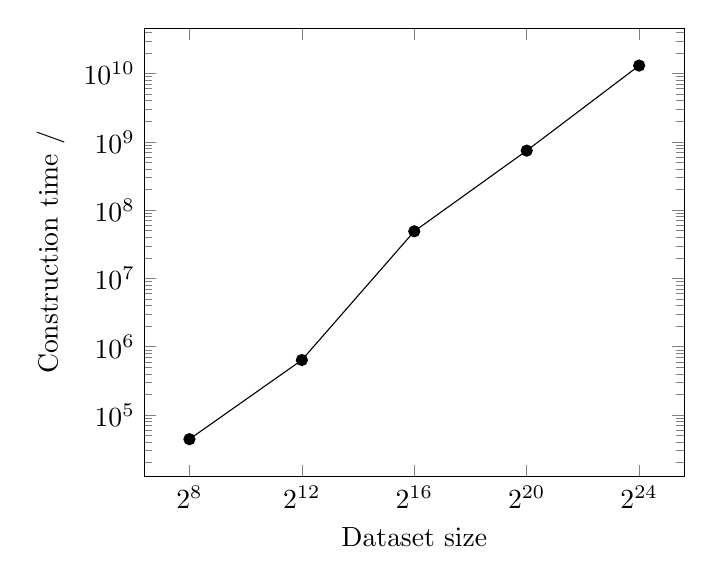
\begin{tikzpicture}
  \begin{loglogaxis}[
    log basis x = 2,
    log basis y = 10,
    xlabel = {Dataset size},
    xtick = {2^8, 2^12, 2^16, 2^20, 2^24},
    ylabel = {\text{Construction time} / \si{\nano\second}},
  ]
    \addplot [mark=*,black] coordinates {
      (256, 44277)
      (4096, 638777)
      (65536, 49027776)
      (1048576, 743982676)
      (16777216, 13091972575)
    };
  \end{loglogaxis}
\end{tikzpicture}
%
  \caption{Relationship between dataset size and summary construction time}
  \label{fig:fingerprint-implementation-performance}
\end{figure}

The results of all \num{25}~runs of each of the five performance tests are presented in \cref{tab:fingerprint-implementation-performance}, and the relationship between the size of a dataset and the time taken to construct its summary is shown in \cref{fig:fingerprint-implementation-performance}.
This relationship appears to be linear, which agrees with the analysis given in \cref{subsec:fingerprint-analysis-complexity}.
Since the update operation has constant amortized time complexity per update, and one update is performed for every item--weight pair in the dataset, the time complexity associated with performing all the updates given in a dataset is linear in the size of the dataset.



\end{document}
